\RequirePackage{snapshot}
\documentclass[10pt,a4paper]{ULBreport}
\usepackage[utf8]{inputenc}
\sceau{Images/sceauULB.jpg}
\graphicspath{ {./Images/} }
\usepackage{multirow}
\usepackage{listings}
\usepackage{color} 
\usepackage{setspace} 
\usepackage{amsmath}

\usepackage{pdfpages}
\usepackage{biblatex}
\usepackage{floatrow}
\usepackage{subcaption} 
\usepackage{siunitx}
\usepackage[many]{tcolorbox}
\usepackage{multirow}
\usepackage{soul}
\usepackage[final]{pdfcomment}
\usepackage{listings}
\usepackage[dvipsnames]{xcolor}
\usepackage{fancyvrb}
\usepackage{hyperref}
\usepackage{xstring}
\usepackage{etoolbox}
\usepackage{svg}

\setcounter{chapter}{-1}

% Colors


% BOXES FOR QUESTIONS

\newtcolorbox{questionBox}[2][]{
    fontupper=\bf,
    boxrule=1.5pt,
    colframe= black, % frame color
    fonttitle=\itshape,
    attach boxed title to top left={yshift=-0.3\baselineskip-0.4pt,xshift=2mm},
    title= #2,#1,
    enhanced,
    }

\newtcolorbox{bonusQuestionBox}[2][]{
    fontupper=\bf,
    boxrule=1.5pt,
    colframe= Peach, % frame color
    colback=Apricot,
    coltitle=black,
    fonttitle=\itshape,
    attach boxed title to top left={yshift=-0.3\baselineskip-0.4pt,xshift=2mm},
    boxed title style={colback=BurntOrange},
    title= #2,#1,
    enhanced,
    }





\begin{document} 


	\titleULB{
	title={Report Lab 3 \\ Virtual Local Area Network (VLAN)},
    studies={IRELE - MA1 Electrical Engineering},
    course ={ELEC-H417},
    author={\textit{Authors :} \\ Amaury ARICO \\ Alexis BOLLENGIER \\ Emmeran COLOT \\Sefa GÖNEN  },
    date={\textbf{Academic year :} \\ 2024 - 2025},
    teacher={\textit{Professor : } \\ Jean-Michel DRICOT \\\textit{Assistant : } \\ Navid LADNER },
    logo={Images/logo-polytech.jpg},
    manyAuthor
	}

\chapter{Mission 0 - Topology}


\section{Bonus question - Lost packet}

\begin{bonusQuestionBox}{Lost packet}
    Do you observe something special with the first (or two firsts) packet of the first ping command ? If yes, what is it and why ? (Wireshark could help)
\end{bonusQuestionBox}


% RESPONSE HERE

\begin{itemize}
    \item \textbf{Routers} operate at \textbf{Layer 3 (Network Layer)} and are used for routing traffic between different networks : \textit{routers are connecting devices from \textbf{different networks} together}. \\ Routers are responsible for determining the best path for data to travel from one network to another one.
    \item \textbf{Switches} operate at \textbf{Layer 2 (Data Link Layer)} and are used for forwarding data within the same network : \textit{switches are connecting multiple devices together within \textbf{one network}}. \\ A switch functions by learning the MAC address of the devices connected to its ports and by forwarding frames based on these addresses. Switches \textbf{do not route traffic}\footnote{Some switches can also do routing (L3), they are known as multilayer switches} between different networks. \\ Also, switches are \textbf{transparent} on the network (the hosts are unaware of the presence of switches) and \textbf{self-learning} (don't need to be configured).
\end{itemize}


\chapter{Mission 1 - VLAN Isolation}

\section{Question - Netmask adaptation}

\begin{questionBox}{Netmask adaptation}
    What should be the netmask to achieve this and why ?
\end{questionBox}


The netmask that should be used to allow PC1 (192.168.20.2) and PC3 (192.168.30.2) to communicate without changing their IP addresses is \texttt{255.255.240.0 (or /20)}.
    
\textbf{Explanation:}\\
We need to find a common part in the subnet portion of both PCs and set the netmask such that the new subnet is this common part.\\
In binary, the IP address \texttt{192.168.20.2} is represented as:
\[
\textcolor{red}{11000000.10101000.0001}0100.00000010
\]
And the IP address \texttt{192.168.30.2} is represented as:
\[
\textcolor{red}{11000000.10101000.0001}1110.00000010
\]
We can see that the first 20 bits of both addresses are the same. That's why the netmask is \texttt{/20 (255.255.240.0)}.

\section{Bonus question - One-way communication}

\begin{bonusQuestionBox}{One-way communication}
    What can you do to make a one way communication (i.e. ping PC1→PC2 works but not PC2→PC1) ?
\end{bonusQuestionBox}



The ping command does \textbf{not work} between PC1 and PC3 after configuring them to be in different VLANs. \\
This is because VLANs isolate traffic at Layer 2, meaning devices in different VLANs cannot communicate with each other unless there is routing in place between them (in our case, no router is configured).



\chapter{Mission 2 - VLAN Trunking}


\section{Question - IPv6 compatibility}

\begin{questionBox}{IPv6 compatibility}
    From PC1, ping Router1 and PC2 IPv4 and IPv6 addresses. What is working ? Why ?    
\end{questionBox}


The figure \ref{trunkICMP} shows the result of a ping command from PC1 to PC2 captured on the trunk line. These PCs are in the same VLAN (VLAN 20) but are physically connected to different switches. \\
As expected, the 802.1Q headers in the ICMP packets contain the tag ID of the VLAN (which is 20).

\begin{figure}[H]
    \centering
    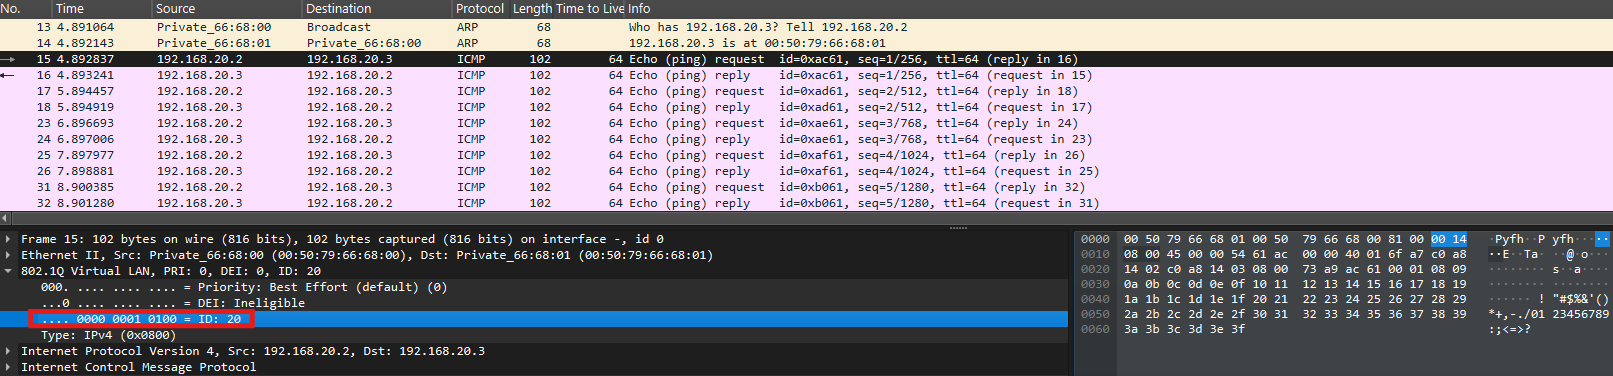
\includegraphics[width=\textwidth]{Images/trunkHeader.png}
    \caption{Wireshark Screenshot - Ping command from PC1 (192.168.20.2) to PC2 (192.168.20.3) in VLAN 20 - Listening to trunk link between Switch1 and Switch2. The tag ID (=20) in the 802.1Q header of an ICMP packet is shown in the red frame.}
    \label{trunkICMP}
\end{figure}



\chapter{Mission 3 - Inter-VLAN Routing}

\section{Question - What is the route}

\begin{questionBox}{What is the route}
    What is the current route (IPs and devices) ? Did the route change (compared to mission 2: RIPv2) and why ?
\end{questionBox}


The ping from PC1 (192.168.20.2 - VLAN 20) to PC4 (192.168.30.3 - VLAN 30) works because of inter-VLAN routing. Even though the two PCs are on different VLANs, the \textit{router on a stick} setup assures the communication between them : the router is forwarding packets between VLAN 20 and VLAN 30, just as a router would between two different LANs.

\par

When PC1 sends a ping request to PC4, the following happens :

\begin{enumerate}
    \item The request reaches Switch1 where its layer 2 header is changed : an 802.1Q header is added below the ethernet header. The tag ID associated with this packet is 20 (this can be seen on the figure \ref{vlan20}).
    \item The request is sent from the Switch1 to the router. When it arrives there, the router changes the tag ID in the 802.1Q header to 30, as shown in the figure \ref{vlan30}. Previously, the request couldn't reach PC4 because it is in VLAN 30 and the request comes from VLAN 20. The goal of the router is to forward the packets from one VLAN to another one.
    \item The router returns the request to Switch1 but this time, because the tag ID is 30, Switch1 handles the request as it was part of VLAN 30. To reach PC4, Switch1 sent the request to the trunk line : Switch2 is connected to PC4. The tag ID is still 30.  
    \item When the request arrives at Switch2, the 802.1Q header is removed and the request is sent to PC4.
    \item The reply follows the opposite path (tag ID 30 until it arrives at the router where it changes to 20)
\end{enumerate}

Concerning the bandwidth : because the router changes the tag ID of the packets, there's twice the amount of packets on the line between the router and Switch1. For example, the ping command generates 5 ping requests. In the figure \ref{vlan20}, we can see that there is 10 ping requests.

\begin{figure}[H]
    \centering
    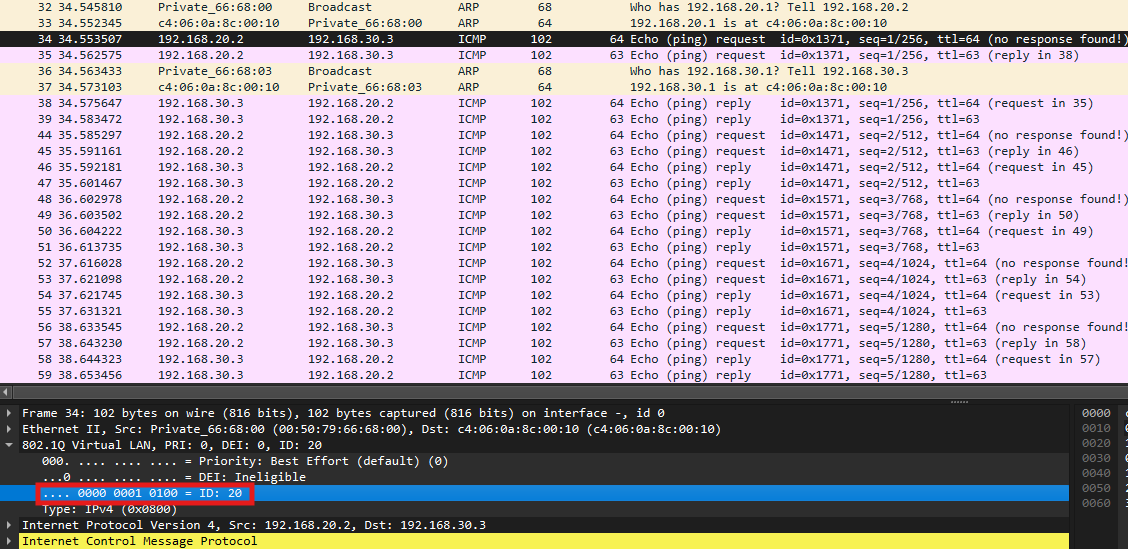
\includegraphics[width=\textwidth]{Images/intervlanID20.png}
    \caption{Wireshark Screenshot - Ping command from PC1 (192.168.20.2 - VLAN 20) to PC4 (192.168.30.3 - VLAN 30) - Listening to link between Switch1 and Router. The tag ID (=20) in the 802.1Q header of one \textbf{ping request} (PC1 $\rightarrow$ PC4) \textbf{before going through the router} is shown in the red frame.}
    \label{vlan20}
\end{figure}

\begin{figure}[H]
    \centering
    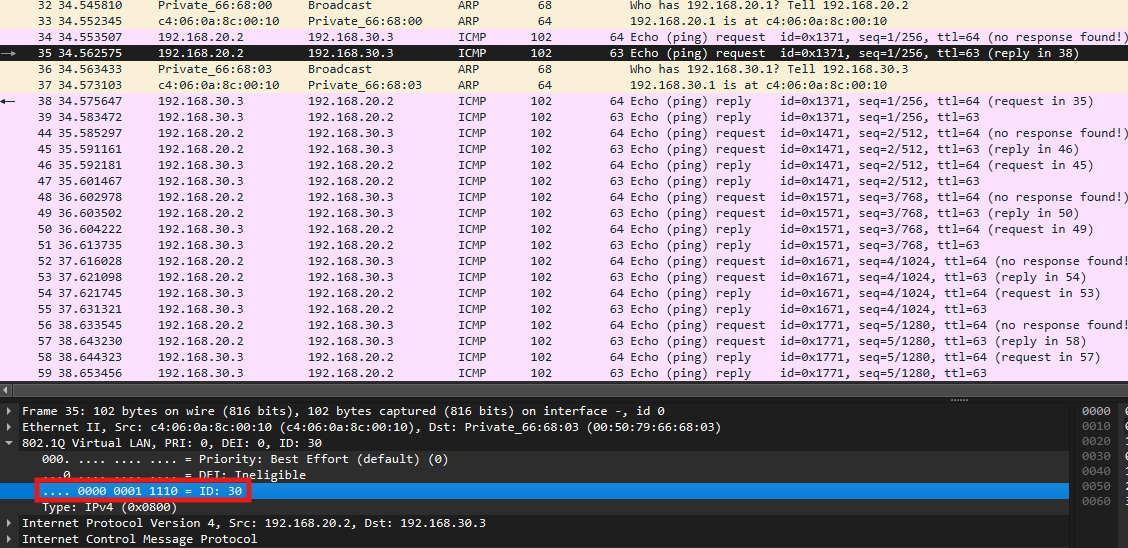
\includegraphics[width=\textwidth]{Images/intervlanID30.png}
    \caption{Wireshark Screenshot - Ping command from PC1 (192.168.20.2 - VLAN 20) to PC4 (192.168.30.3 - VLAN 30) - Listening to link between Switch1 and Router. The tag ID (=30) in the 802.1Q header of one \textbf{ping request} (PC1 $\rightarrow$ PC4) \textbf{after going through the router} is shown in the red frame.}
    \label{vlan30}
\end{figure}

\section{Bonus question - VPN Security}

\begin{bonusQuestionBox}{VPN Security}
    Is VPN really a good way to secure your communication ? Why ? If it is not the case, what could you do instead (or in addition) ?
\end{bonusQuestionBox}


The laboratory investigation into VLANs focused on three principal areas of inquiry. The key areas of focus were \textbf{VLAN isolation}, \textbf{VLAN trunking}, and \textbf{inter-VLAN routing}.

\begin{itemize}
    \item The demonstration of \textbf{VLAN isolation} illustrated the efficacy of establishing discrete VLANs to restrict communication between devices at \textit{Layer 2}, enhancing security and optimizing traffic management. This demonstrated the importance of segmenting network traffic to enhance efficiency and security.
    \item \textbf{VLAN trunking} allows devices that are \textit{physically apart} and connected to different switches to be \textit{logically} connected within the same network.
    \item \textbf{Inter-VLAN} routing was implemented through a \textit{router on a stick} configuration, wherein the router assured communication between devices situated within disparate VLANs by forwarding packets through its subinterfaces. This demonstrated how inter-VLAN routing enables cross-VLAN communication while maintaining the logical separation provided by VLANs.
\end{itemize}

Overall, the lab highlighted the important role of VLANs in designing scalable, efficient, and secure networks. Through VLAN isolation, trunking, and inter-VLAN routing, the lab illustrated how VLANs are used to segment, extend, and interconnect network traffic in modern network designs.

The figures \ref{Mission2} and \ref{Mission3} show the schema of the topology after mission 2 and 3.

\begin{figure}[H]
    \centering
    \includesvg[width=1\textwidth]{Mission2.svg}
    \caption{Schemas of the physical and logical topology after mission 2}
    \label{Mission2}
\end{figure}

\begin{figure}[H]
    \centering
    \includesvg[scale=0.6]{Mission3.svg}
    \caption{Schemas of the physical and logical topology after mission 3}
    \label{Mission3}
\end{figure}

\section{Question - What changes in the routing table after a network link failure ?}

\begin{questionBox}{What changes in the routing table after a network link failure ?}
    Display the routing table of your routers. What have changed ? How much time has it taken to change ? What could happen if you do a ping between PC1 and PC2 before the changes takes place ? What is the current route and its length ? Did the route change and why ?
\end{questionBox}

Inter-VLAN routing provides several opportunities for enhancing security. One key benefit is \textbf{traffic segmentation}: by isolating different types of traffic into separate VLANs, you can limit access to sensitive data (like limiting the range of broadcasts from layer 2 : ARP, DHCP, MAC addresses,...) and restrict communication between devices that do not need to communicate. \par
Another advantage is the use of Access Control Lists. Routers can be configured with ACLs to control which devices or networks can access other VLANs, allowing for more granular security policies between VLANs.

% However, a security threat such as \textbf{VLAN hopping} can occur when a malicious user gains unauthorized access to another VLAN, usually by exploiting trunk ports. This can be mitigated by securing trunk ports with proper VLAN tagging and using private VLANs to prevent unauthorized traffic from hopping between VLANs.
\end{document}

% frame.number >= && frame.number <=
